\begin{figure}[H]
  \centering
    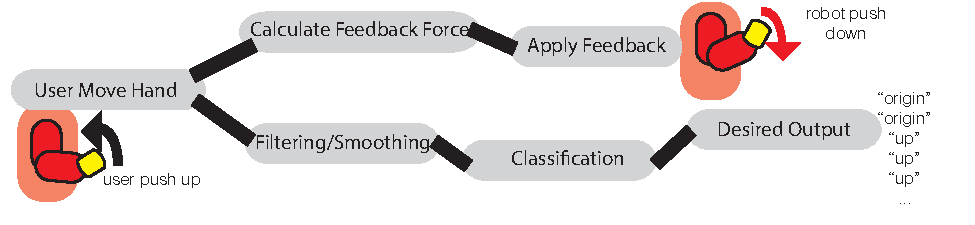
\includegraphics[width=\textwidth]{graph1}
  \caption{System flowchart shows how the the user's action(left) flows through our pipeline to calculate the required feedback force and infer the correct action.}
  \label{fig:sys}
\end{figure}
The system mainly consist of two parts, a feedback system and an action classifier. A flowchart showing the system design is shown above in figure \ref{fig:sys}. The system was built for the Baxter Research Robot \footnote{http://www.rethinkrobotics.com/baxter-research-robot/} that uses the Robot Operating System(ROS) \footnote{http://www.ros.org/}. However, we believe that the system can be easily extended to other robotic platforms with active compliant actuators. Baxter has two 7 degree of freedom arms with compliant actuators. Descriptions of both parts of the systems are as following:


\subsection{Feedback System}
The first part of the system simulates the physical property of a joystick where the arm will try to return to the resting position and apply greater force the further it is away from the resting position. We do this through attaching virtual springs at each joints. The springs are modeled using Hooke's law \cite{wiki:hooke}, which is the first-order approximation of the stress-strain relationship of a spring. Hooke's law is described as:
\begin{equation}
F = -kx
\end{equation}
where k is the spring constant and $x$ is the change in length of the spring. The relationship could also be described by the general stress and strain relationship
\begin{equation}
\sigma = Y \epsilon
\end{equation}
Where $\sigma$ is the stress, $\epsilon$ is the strain and $Y$ is the Young's modules which describes the linear relationship between stress and strain. Our model does not model the yield point which is the point in the physical world where the relationship between stress and strain is no longer linear.

In our system, Hooke's law is applied on every single joint(7 per arm) on the robot where $x$ is defined as the change of radian from the resting position and $k$ was selected from trial and error. The selection of $k$ for each joint was also influenced by movement restriction we wanted to imposed such as making actuators further away requiring more force to move. These restrictions where selected to make the classification process easier.
However if we only applied Hooke's law, when the user release the hand, the arm will actually oscillate between points without any resistance(since the springs are virtually applied, real life physical resistance like air and loss of energy doesn't exist). To address this, a damping force \cite{wiki:damping} is applied to the system which is described with the following equation.
\begin{equation}
F = cv
\end{equation}
where $c$ is the damping coefficient and $v$ is the velocity of the system. Through damping, we could also simulate a useful physical property of an oscillating system called \textbf{critically damped} which is the state where the system will return to the resting position as fast as possible without any oscillation. A critically damped system is a system where the damping ratio, $\zeta$ is equal to 1. The damping ratio of the system is calculated with
\begin{equation}
\zeta = \frac{c}{2\sqrt{mk}}
\end{equation}
However, we do not know the actual mass of each individual component of the system, instead, the damping coefficient,$c$ was calculated through trial and error until oscillation is no longer observable.


\subsection{Classification}
\subsubsection{Filtering}
Before classification methods were applied, we applied a common noise filtering algorithm, Exponentially Weighted Moving Average(EWMA) on the raw input data to smooth out the existing noise due to sensor errors. The filtering equation is defined as
\begin{equation}
x_t = \alpha y_{t-1} + (1 - \alpha)x_{t-1}
\end{equation}
where $x_t$ is the filtered data at each time step, $y_t$ is the raw input data at each time step and $x_{t-1}$ is the filtered input at the previous time step. $\alpha$ is the control parameter that select which number to be weighted more. In our study, we selected $\alpha$ to be $0.25$ through trial and error.\\

\subsubsection{Feature Selection}
We selected 14 different features that were used for the classifications. The features were the actual torque applied on each joint(one for each seven joints) and the position of the actuators in radian(one for each seven joints). The actual torque is different from the commanded torque in each command cycle as it also measures the torque that is applied on the system by external forces like the user pushing the arm in a certain direction. We choose not to use the end effector coordinates as a feature as we believe possible information gain in the 3D coordinate are already captured by our features.

\subsubsection{Planned Output}
We designed our system with the hope to distinguish 7 different actions that the user could perform, \textbf{upwards}, \textbf{downwards}, \textbf{left}, \textbf{right}, \textbf{forward}, \textbf{backwards} and finally \textbf{origin}.

\subsubsection{Training Data}
Training data for the classification was constructed with one member of the research team moving the robot arm with different actions and recording the values in the feature space at the end of each action. Each sample is then manually labeled with their respective actions by the same member.

\subsubsection{Classification Algorithms}
Because the way motion worked and the problem space, we believed the different actions are linearly separable to each other(they might be not linearly separable to all) in our feature space. We selected a few different classification methods that benefit from this property and compared their performance. We used the python machine learning library, scikit-learn \footnote{http://scikit-learn.org} in our implementation of the system.

\paragraph{K-Nearest Neighbor Algorithm}
K Nearest Neighbor finds the $K$ number of nearest point in the training data and picks the most common action in the nearest points with the distance as their weights. For our usage, the algorithm relies on using K-d tree structure, which is a binary tree where each node separates the high dimension space into 2 to optimize the search. In our study, $K$ was set to 5 through trial and error.

\paragraph{Logistic Regression} 
Logistic Regression is a linear model of the data and uses the following logistic function to calculate the probability for each action.
\begin{equation}
f(x) = log(1 + e^{-y_iw^Tx_i)})
\end{equation}
where $x$ is the sample, $y$ is the label and $w$ is the weights of the linear model. The goal of the Logistic Regression is to find the weights that minimize the difference between logistic function and the training data labels. This can be expressed as the following minimization problem.
\begin{equation}
\min_w ||w||_1 + C\sum_{i=1}^l log(1 + e^{-y_iw^Tx_i)})
\end{equation}
Where C is the penalty of the error to prevent over fitting. The formulation and description of the used algorithm in the library can be find in \cite{Fan08}.

\paragraph{Support Vector Machines}
The final method tried is Support Vector Machines with soft margins \cite{cortes1995} that uses a linear kernel. The formulation of the problem is similar as we have done in homework 4. Where we tried to maximize the margin by solving the following constrained optimization problem: 
\begin{equation}
\begin{aligned}
& \min_{w,b,\epsilon} \frac{1}{2} w^Tw + C \sum_{i=1}^n \epsilon_i\\
& \text{such that}\\
& y_i(w^Tx_i + b) \leq 1 - \epsilon_i, \forall i\\
& \epsilon_i \geq 0, \forall i
\end{aligned}
\end{equation}
Again, the algorithm we used solve the minimization problem through transforming the problem to the Lagrange function similarly to homework 4. 